\section{Redes neuronales profundas}

TODO

\subsection{Redes neuronales convolucionales}

\noindent
En 1989, el francés Yann LeCun comenzó a trabajar en los fundamentos de un novedoso modelo\
neuronal basado en la biología de la corteza visual del cerebro animal. Su trabajo, eventualmente,\
lo llevó a ser nombrado director de la investigación en IA en Facebook. Su ascenso\
al \emph{``podio''} del aprendizaje profundo es producto de una revolución en la\
\emph{vanguardia} del reconocimiento de imágenes a través de computadoras. Y lo más probable\
es que el mismo modelo continúe sobresaliendo por algunos años.\par
Como la mayoría de las arquitecturas neuronales, las \textbf{redes neuronales convolucionales}\
(\emph{CNN's}, por sus siglas en inglés) no alcanzaron la popularidad suficiente hasta entrada\
la época reciente, caracterizada por una alta conectividad (a través de Internet) y un incremento\
significativo en la capacidad de cómputo de los dispositivos modernos. Sin embargo, LeCun ya había\
obtenido resultados sobresalientes hacía 1998, en tareas de reconocimiento de patrones \cite{bengio2009}.\
El enfoque de LeCun, y de su equipo en \emph{Bell Labs}, consistió en dar un modelo de mayor\
capacidad en \emph{representaciones internas} que el tradicional perceptrón multicapa.\par
Un aspecto importante en esta arquitectura consiste en la delegación de ciertas partes de la misma\
a sub-problemas específicos de la tarea a resolver. Por consiguiente, cada capa de una CNN definirá\
uno (o varios) niveles de representación, los cuales capturan ciertas características inherentes\
al flujo de datos de entrada. Mediante un basto conjunto etiquetado de datos, se pueden aprender dichas\
abstracciones de manera supervisada.

\subsubsection{La capa convolucional}

Para iniciar la discusión sobre la estructura de una CNN, usaremos como ejemplo al reconocimiento\
computacional de imágenes; sin embargo, cabe notar que esta arquitectura es popular en tareas donde\
exista la necesidad de reconocer patrones sobre conjuntos de datos con topología \emph{cuadriculada}.\
\footnote{De acuerdo a \cite{goodfellow-et-al-2016}, como ejemplos de datos con una topología cuadriculada,\
  se incluyen series de tiempo (cuadrícula de una dimensión), audio o videos.}
Uno de los conjuntos de datos más famosos, y de mayor tradición, es la \emph{Mixed National Institute of Standards}\
\emph{and Technology database}, mejor conocida como MNIST. En ella se alberga una gran cantidad de dígitos\
escritos a mano; el problema, entonces, consiste en clasificar cualquier manuscrito dado en una de las $10$ clases\
existentes, de acuerdo al dígito más parecido.\par

\begin{figure}
  \centering
  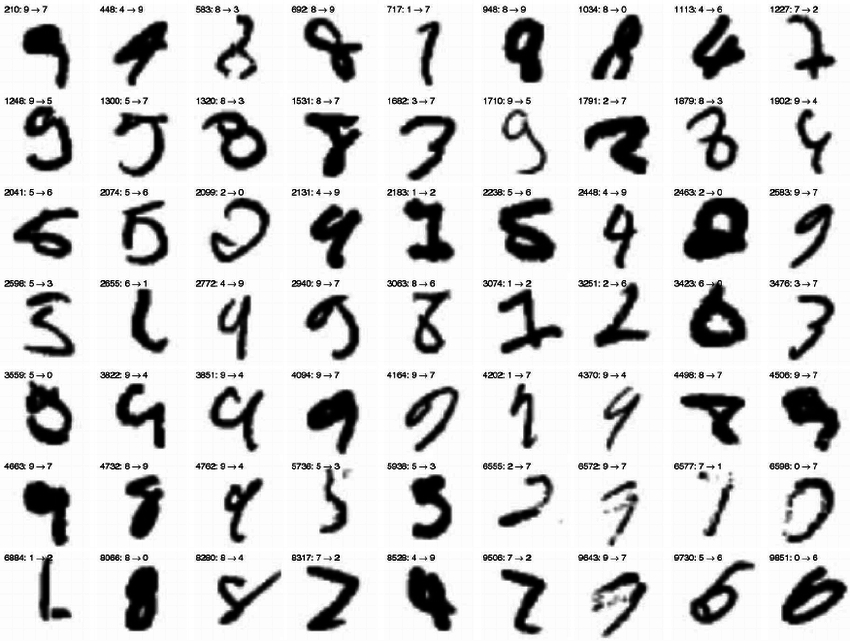
\includegraphics[width=0.6\textwidth]{mnist}
  \caption{Algunos dígitos existentes en la base de datos MNIST.
    (Tomado de \url{http://www.researchgate.net/}.)}
  \label{mnist_fig}
\end{figure}

Como se observa en la figura (\ref{mnist_fig}), existen distintas maneras de escribir a mano un solo dígito. Quisiéramos\
que nuestra solución sea lo suficientemente robusta para distinguir $4$'s de $9$'s por más ilegible que\
sea la letra. No tenemos idea de dónde buscar ciertas características o si el observar un cambio drástico\
en el color de varios pixeles contiguos nos sea significativo; todo esto es parte de lo que se deberá de\
\emph{aprender}. Esta incertidumbre en la detección de atributos conduce a, de alguna manera, ir en\
búsqueda de pequeñas porciones de la imagen que nos den una pista por dónde empezar.\par
En este punto cabe recordar que usualmente para una computadora, una imagen es un arreglo de tres dimensiones,\
cada una especificando la posición de un pixel y su color. En la práctica (y de acuerdo a las últimas tendencias\
de programación de redes neuronales), a esta estructura se le llama \textbf{tensor}, por lo que seguiremos\
la convención. Volviendo a nuestra búsqueda, necesitamos un parámetro que nos indique el mínimo de pixeles a\
analizar para empezar a encontrar detalles claves de la imagen. Por ello, vamos a usar un pequeño tensor ``cuadrado''\
para recorrer toda la imagen. A dicho tensor le llamaremos \textbf{filtro} (\emph{kernel}, en inglés).\
Llamaremos \textbf{zancada} (\emph{stride}, en inglés) al número de pixeles que ``saltamos'' (en cualquier dimensión)\
al mover un filtro sobre la imagen. La salida se calcula realizando una combinación lineal sobre cierta región de la\
imagen ponderada con los valores del filtro y añadiendo un sesgo. Esto produce un tensor con una profundidad\
equivalente al número de filtros usados. En símbolos, esto corresponde a realizar lo siguiente
\begin{equation} \label{entry-wise-sum}
  \sum _{i} x_i w_i\ + b
\end{equation}
donde $x_i$ y $w_i$ corresponden a la $i$-ésima entrada de la imagen y del filtro, respectivamente, y $b$ es el sesgo.\par
En ocasiones es conveniente rodear una imagen con ceros, ya que debemos garantizar que el filtro encaje\
exactamente dentro de la imagen conforme se va deslizando horizontal y verticalmente. A esto se le conoce como\
\textbf{relleno de ceros} (\emph{zero-padding} en inglés). Los parámetros que acaban de ser presentados\
constituyen a una \textbf{capa convolucional}, en la cual reside la mayor carga computacional de la arquitectura.\
Para abreviar, en adelante nos referiremos a dicha capa con la sigla \textbf{CONV}.\par
La correcta elección de parámetros debe de garantizar que el filtro no salga de las dimensiones de la imagen\
de entrada (sujeta a relleno de ceros). Supongamos que tenemos una imagen cuadrada de dimensión $W \times W$,\
un filtro de dimensión $F \times F$. Además ``enmarcamos'' (rellenamos) de ceros la imagen con un grosor de $P$\
pixeles y aplicamos el filtro con una zancada $Z$. Entonces, la cantidad de neuronas resultantes (en una dimensión)\
está dada por
\begin{equation}
  \frac{W - F + 2P}{Z} + 1,
\end{equation}
donde este número es un entero positivo.

TODO: Ejemplos con imágenes

\subsubsection*{La \emph{convolución}}

\noindent
Matemáticamente, este proceso se puede formalizar mediante la convolución de dos funciones reales.\
Si $x$ denota a nuestro dígito desconocido y $w$ a nuestro filtro, entonces la convolución de $x$ con\
$w$, en un punto $t$, se define como:
\begin{equation}
  c(t) := \int x(a) w(t-a) da
\end{equation}
y se denota:
\begin{equation}
  c(t) = (x * w)(t).
\end{equation}
En el mundo digital, tenemos conjuntos de datos discretos, por lo que es conveniente dar una definición\
adaptada al respecto:
\begin{equation}
  c(t) = (x * w)(t) := \sum _{a=-\infty} ^{\infty} x(a) w(t-a).
\end{equation}
Dentro del contexto de reconocimiento de imágenes, es útil especificar que la convolución se hace en dos\
dimensiones de las que se están contemplando. Para ello introducimos la siguiente notación:\
si $i$ y $j$ son valores que denotan la posición de un pixel, $X(i,j)$ es el valor (color) correspondiente\
y $K(i,j)$ denota la entrada $(i,j)$ de nuestro filtro, definimos a la convolución $C$ como:
\begin{equation}
  C(t) = (K * I)(i,j) := \sum_m \sum_n I(i-m,j-n) K(m,n).
\end{equation}
Muchas bibliotecas de redes neuronales utilizan la \textbf{correlación cruzada} en vez de la convolución.\
Semánticamente, la correlación cruzada sirve para analizar lo mismo que buscamos con la convolución; por\
ello, esta sutil distinción muchas veces no es notada. La definición es la siguiente:
\begin{equation} \label{cross_corr}
  C(t) = (I * K)(t) := \sum_m \sum_n I(i+m,j+n) K(m,n).
\end{equation}
Nótese que en las dos últimas definiciones se ha convenido \emph{voltear} los índices del filtro. En la\
teoría, la ventaja que trae esto consiste en una mayor facilidad de probar ciertos resultados.\par
Para terminar de describir la \textbf{capa convolucional} de la arquitectura,\
vale la pena hablar un poco sobre la salida de (\ref{cross_corr}). Aquí estamos\
caracterizando al valor de cada neurona como se describió en (\ref{entry-wise-sum}).\
Al conjunto de tensores resultantes se les conoce, convenientemente, como \textbf{mapas de activación}.\par
Cabe señalar que la eficiencia de la convolución es mucho mayor a la de una\
multiplicación de matrices (en una capa densa) y esto ocurre, principalmente, por las siguientes razones:
\begin{itemize}
\item En una capa densa, se consideran interacciones entre cada neurona de entrada con cada neurona de salida.\
  Es decir, los productos matriciales involucran a cada pixel, sin importar qué lugares en específico son\
  los que vale la pena resaltar.
\item Se dice que en una capa convolucional se manejan \textbf{pesos esparcidos}, los cuales corresponden\
  a las entradas del filtro. Esto significa que después de un entrenamiento, el filtro aprenderá a interactuar\
  con ciertos grupos de pixeles, sin conocer su distribución. Con esto es posible tomar en cuenta pequeños\
  detalles que ocurren en una vecindad reducida de pixeles.
\item En una capa convolucional, los pesos del filtro que se buscan aprender son mucho menos que los pesos que\
  se aprendería en una capa densa: si la imagen de entrada contiene miles o millones de pixeles, entonces\
  necesitamos cientos de pixeles en nuestro filtro para aprender los razgos más pequeños de la misma (como\
  bordes o puntos).
\end{itemize}\par
En resumen, si tenemos $m$ entradas y $n$ salidas en una capa, y ésta es densa, entonces habremos de realizar\
$O(m \times n)$ operaciones para calcular la salida. En cambio, en una capa convolucional, podemos tener\
una zancada $k$ de pixeles en el filtro, con un orden de magnitud mucho menor a $n$; lo cual va a provocar\
que sea más eficiente calcular $O(m \times k)$ operaciones.

\subsubsection*{Filtros vistos como arreglos de neuronas}

\noindent
Dependiendo del número de filtros escogidos para aplicarse en la capa CONV, se definirá la salida de la misma.\
Intuitivamente, si se usan $12$ filtros en una imagen cuya dimensión de entrada es de $32 \times 32 \times 3$,\
un puede imaginarse $12$ imágenes procesadas por la capa CONV, como resultado del procesamiento REF-IMAGEN.\
Es decir, la dimensión de la salida sería de $32 \times 32 \times 12$.\par
Esto no corresponde al ``mecanismo canónico'' que caracteriza a una capa neuronal, en donde todas las entradas\
participan en la decisión de la salida. Más aún, a diferencia del perceptrón multicapa, en donde el aprendizaje se\
da ajustando los pesos de cada \emph{sinapsis}, aquí cada neurona tendrá asociado un peso que será ajustado.\
Sin embargo, podemos ahorrarnos la discusión sobre cómo adaptar al algoritmo de propagación hacia atrás para\
hacer que cada neurona aprenda, transformando un poco la arquitectura:
\begin{itemize}
\item Si nuestra dimensión de entrada es de $32 \times 32 \times 3$, ``aplanamos'' dicho tensor de manera vertical,\
  es decir, en uno de dimensión $1024 \times 1 \times 3$.
\item Por cada filtro, apilamos todas las neuronas en una salida cuya altura está determinada por el valor de la zancada.
\item Cada neurona de salida estará conectada a tantas neuronas de entrada como indique, otra vez, la zancada. Éstas\
  serán contiguas tras ser transformadas como indica el primer punto mencionado. Adicionalmente, podemos pensar\
  que todas las demás neuronas de entrada están conectadas a cada salida con un peso equivalente a cero unidades.
\item En este caso, los valores que constituyen al tensor de filtro estarán codificados como pesos en cada sinapsis.
\item La $i+1$-ésima neurona de salida tendrá como primera entrada (en orden de arriba hacia abajo), a la segunda\
  entrada de la $i$-ésima neurona.
\end{itemize}\par
La capa de salida de este reacomodo corresponde a un mapa de activación ``aplanado''. Si queremos un \emph{volumen}\
de salida con 12 mapas, entonces habrá que visualizar un modelo en el cual tenemos 12 mapas aplanados conectados, cada uno,\
al tensor de entrada y sin sinapsis alguna entre cada uno de éstos. Cabe destacar que durante el entrenamiento,\
basta actualizar únicamente un solo conjunto de pesos que conectan a una neurona de salida con una cantidad de entradas\
equivalente al valor de la zancada y, posteriormente, propagar los nuevos valores a los demás pesos por cada neurona de\
salida; esto por cada uno de los filtros. Esto ocurre debido a que cada uno de los filtros \emph{``comparte parámetros''},\
como se observa en la figura \label{fCNN_fig}.

\begin{figure}
  \centering
  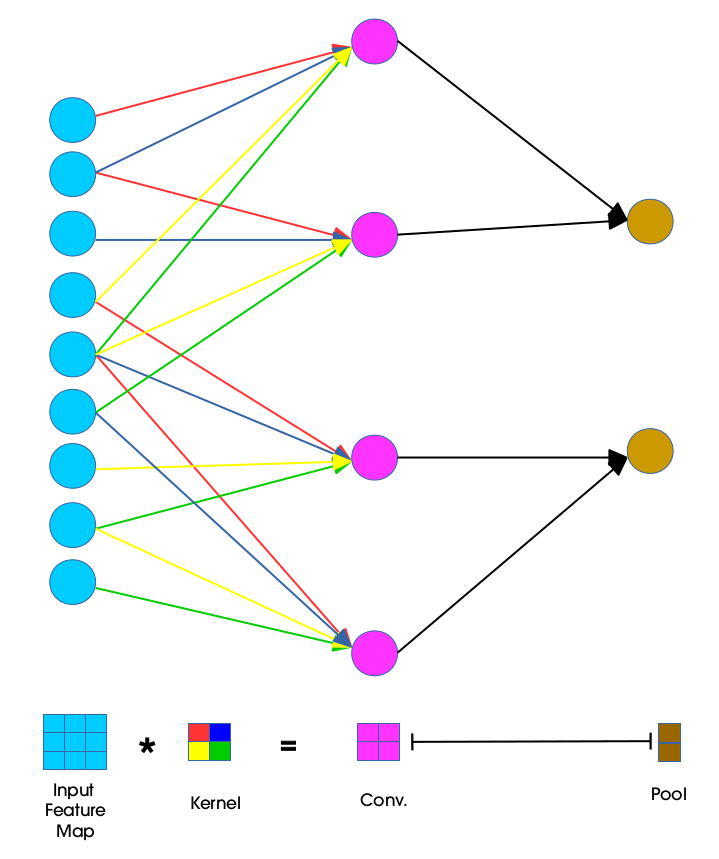
\includegraphics[width=0.65\textwidth]{fCNN}
  \caption{El concepto de pesos compartidos. Las sinapsis del mismo color representan conexiones con pesos iguales.
    En este caso, se tendría una zancada de 4 neuronas.
    (Tomado de \url{http://www.jefkine.com/general/2016/09/05/backpropagation-in-convolutional-neural-networks/}.)}
  \label{fCNN_fig}
\end{figure}

\subsubsection*{La \emph{``capa''} de activación}

\noindent
Como sucede al calcular las salidas de una capa densa, aquí hay que utilizar una función no lineal (y \emph{suave}) para\
finalizar la clasificación. En algunos casos, a este paso se le suele llamar \textbf{capa de no linealidad}.\
En \cite{lecun2010}, además de usar dicho término, se propone a la función $tanh$, sobre cada entrada de los\
mapas de activación, como el estándar en CNN's. Sin embargo, también se señala que una \emph{sigmoide}\
\emph{rectificada} ha dado buenos resultados en reconocimiento de imágenes (sujeta a una normalización posterior);\
el caso particular es el de la \textbf{unidad lineal rectificada} (\emph{ReLU}, por sus siglas en inglés):
\begin{equation}
  f(x) = \max(0, x).
\end{equation}

\begin{figure}
  \centering
  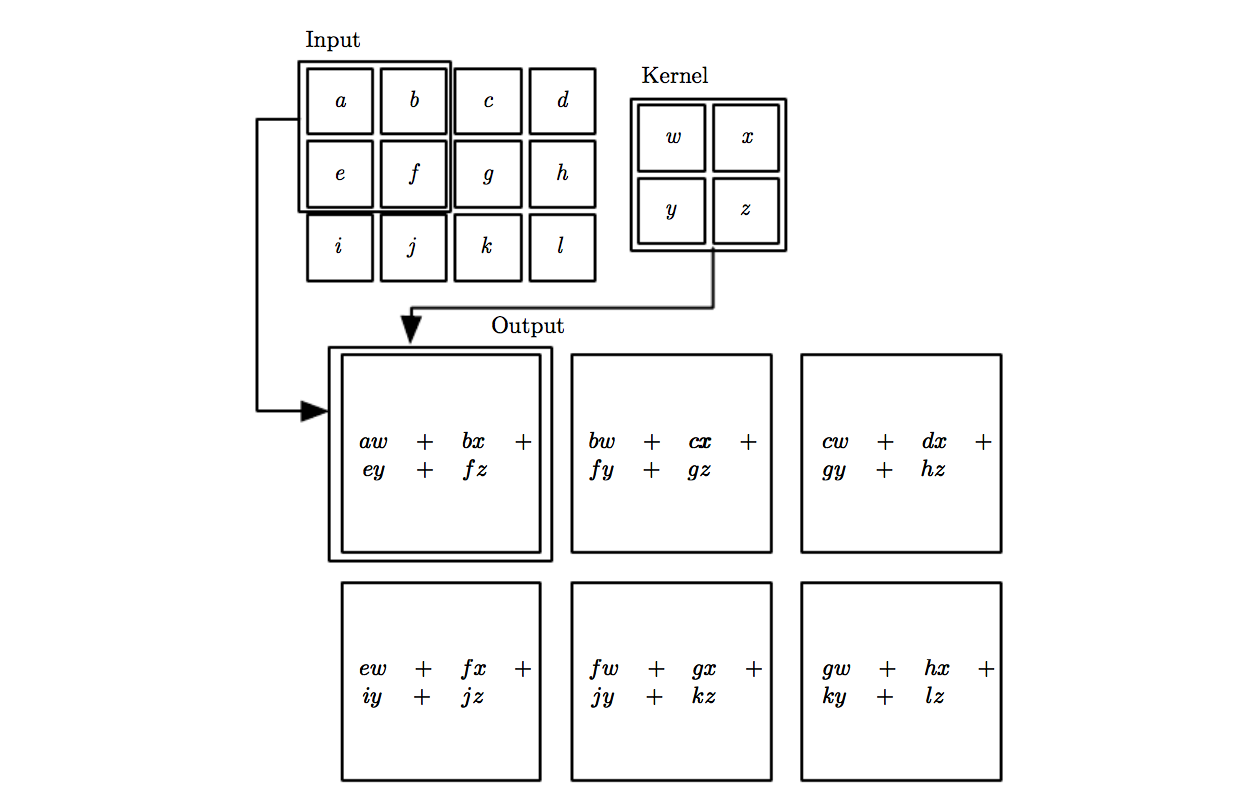
\includegraphics[width=0.9\textwidth]{2dconv}
  \caption{Ilustración del proceso de convolución. El filtro se desliza por la imagen de entrada y
    se efectúa un producto pixel por pixel.)
    (Tomado de \cite{goodfellow-et-al-2016}.)}
  \label{2dconv_fig}
\end{figure}

\subsubsection*{La capa de \emph{pooling}}

\noindent
Un exceso de aprendizaje en la capa de convolución puede provocar un \emph{sobreajuste} sobre\
el modelo. Esto se puede observar, en nuestro ejemplo, con una arquitectura donde cada filtro\
se entrene a funcionar para un grupo pequeño y exclusivo de pixeles, los cuales esperen encontrar\
detalles claves en lugares precisos. Es necesario, entonces, ocuparse de que una CNN\
\emph{generalice} suficientemente su aprendizaje para aumentar su robustez.\par
Por ello, las CNN's llevan, además de capas convolucionales, algunas capas de \textbf{agrupación}\
(\emph{pooling}, en inglés y usaremos esta palabra en adelante) con las cuales se puede extraer\
los detalles más fundamentales de cada mapa de activación. En la práctica, existen dos operaciones\
de pooling que sobresalen sobre las demás: \emph{max}-pooling y \emph{avg}-pooling. Para calcular cualquier\
capa de pooling, se define una vecindad en cada mapa de activación (que no exceda su zancada);\
acto seguido, dependiendo del pooling a usar, se almacena el máximo o el promedio de los pixeles\
abarcados en la vecindad.\par
Con esta capa, la arquitectura convolucional se vuelve \textit{aproximadamente \emph{invariante}} a modificaciones\
en la entrada. Esto nos permite enfoarnos más en la existencia de ciertas características en la imagen\
que en la posición exacta de las mismas.\par
El pooling, además, nos brinda un mecanismo de disminución de parámetros del modelo (neuronas)\
brindando la posibilidad de optimizar mucho más la memoria utilizada y las dimensiones de las capas.

\begin{figure}
  \centering
  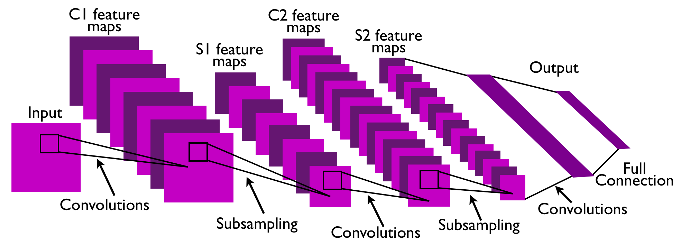
\includegraphics[width=0.8\textwidth]{convnet}
  \caption{Estructura básica de una red neuronal convolucional, con dos fases de extracción de características.
    (Tomado de \cite{lecun2010})}
  \label{convnet_fig}
\end{figure}


\subsection{Redes neuronales recurrentes}

\noindent
Es frecuente encontrar situaciones en las que exista un orden secuencial entre los datos de entrenamiento.\
Esto es algo que tienen en común tareas como reconocimiento del habla o traducción automática (de idiomas).\
Aquí cada instancia de un conjunto de datos se puede ver como una sucesión de valores
\[\mathbf{X} = \mathbf{x}^{(1)},\ldots,\mathbf{x}^{(\tau)}\]
y el objetivo es entrenar una arquitectura que nos permita predecir $\mathbf{x}^{(i+1)}$,\
dados $\mathbf{x}^{(1)},\ldots,\mathbf{x}^{(i)}$.\par
Un modelo (\emph{estadístico}) de lenguaje es una función de probabilidad sobre cualesquiera sucesiones de símbolos\
de un alfabeto dado. En procesamiento de lenguaje natural (\textbf{PLN}), la construcción de estimadores que tengan la capacidad\
de estructurar oraciones dado un conocimiento \emph{a priori} ($\mathbf{x}^{(1)},\ldots,\mathbf{x}^{(i)}$),\
es decir, maximizar
\begin{equation}
  P(\mathbf{x^{(i+1)}}\ |\ \mathbf{x}^{(1)},\ldots,\mathbf{x}^{(i)}).
\end{equation}
El lenguaje natural es inherentemente ambiguo; hecho que ha popularizado el enfoque probabilístico en PLN, dejando\
atrás arquitecturas puramente simbólicas cuya capacidad de cómputo es limitado. Por ejemplo, el enunciado\
\emph{``Eutropio acomodó el portafolio que Porfirio tiró en el buró''} se puede interpretar de dos maneras:
\begin{itemize}
\item Eutropio encontró el portafolio en el buró y procedió a acomodarlo en algún otro lugar.
\item Porfirio dejó tirado el portafolio; acto seguido, Eutropio lo colocó en el buró.
\end{itemize}\par
En un modelo de lenguaje, ¿cómo decidimos qué interpretación semántica tomar? En la práctica, esto depende del\
contexto (conjunto de datos) y la tarea específicamente a resolver. En términos formales, existe más de un\
\emph{árbol de análisis sintáctico} que caracteriza al enunciado anterior y el modelo debe de encontrar qué árbol tomar\
como interpretación.\par
La teoría de lenguajes formales establece que la elaboración de árboles sintácticos, de gramáticas no ambiguas, es un proceso que requiere\
un modelo computacional que necesariamente utilice al menos una \emph{memoria temporal}. Pero, en general, la ambigüedad\
semántica nos obliga a no poder acotar el tamaño de dicha memoria, por lo que necesitamos una arquitectura \emph{turing-completa}\
al menos para fines de construcción de enunciados sintáctica y semánticamente correctos.\par
Un \textbf{red neuronal recurrente} (\emph{RNN}, por sus siglas en inglés) es una arquitectura que posee una memoria interna.\
La estructura básica de la misma se muestra en la imagen REF-IMAGEN. Podemos observar que la estrategia gráfica para incorporar\
a dicha memoria consiste en establecer un \emph{ciclo} entre la salida y la entrada, es decir, existirá una matriz de pesos que se entrenará y guardará\
un resumen de los aspectos importantes de cada símbolo de la sucesión $\mathbf{X}$ que va procesando.

\begin{figure}
  \centering
  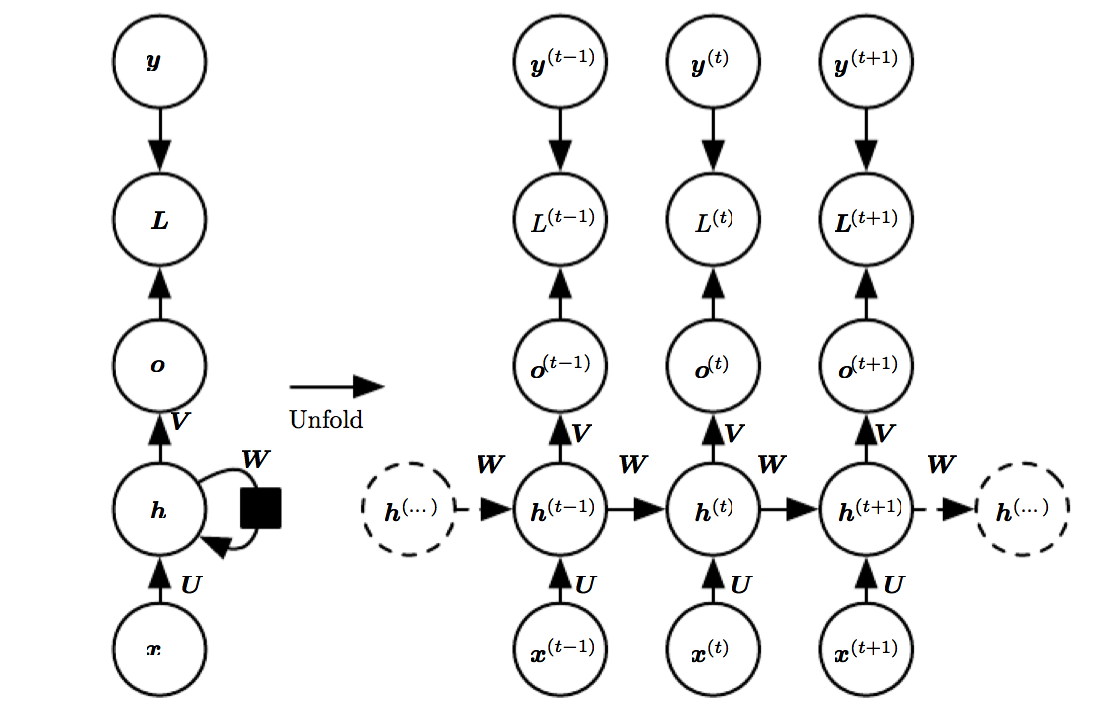
\includegraphics[width=\textwidth]{rnn}
  \caption{Estructura de la compuerta cerrada de una LSTM.
    (Tomado de \cite{goodfellow-et-al-2016})}
  \label{convnet_fig}
\end{figure}

Antes de proceder con el funcionamiento de una RNN, es importante hablar sobre por qué una CNN no es un modelo adecuado\
para el procesamiento de datos secuenciales. La filosofía del procesamiento de imágenes en aprendizaje profundo consiste\
en aprender a reconocer patrones que caractericen a la instancia dada, muchas veces sin importar las relaciones que existan\
entre ellos mismos. Sin embargo, es inconveniente dejar de lado estas relaciones, pues la estructura gramatical\
del lenguaje natural implica un orden que es difícil de capturar por una CNN: habría que compartir parámetros (sinápsis)\
entre capas convolucionales. Más aún, dejando de lado el proceso de entrenamiento, una CNN es una máquina finita de estados\
que carece de una memoria temporal, pues la información solo fluye ascendentemente entre capas\
ignorando un posible retroalimentación de lo que se aprendió con $\mathbf{x}^i$ al momento de procesar $\mathbf{x}^{i+1}$.

\subsubsection*{¿Cómo funciona la arquitectura recurrente?}

\noindent
Como se mencionó anteriormente, la memoria interna de una RNN se codifica con una matriz de pesos. Se dice que estos parámetros\
se \emph{comparten} a través del tiempo, conforme la red va procesando la secuencia de entradas. Formalmente,\
escribimos este fenómeno bajo la intuición de un sistema dinámico, en el que en un tiempo $t$, el estado actual del mismo depende del\
anterior, de la entrada actual y de los parámetros del sistema:
\begin{equation} \label{recurrence-eq}
  \mathbf{h}^{(t+1)} = f(\mathbf{h}^{(t)}, \mathbf{x}^{(t+1)}; \mathbf{\theta}).
\end{equation}
Se puede pensar que la función $f$ determina qué aspectos del pasado son lo suficientemente importantes para predecir el futuro.\
Cabe observar que $f$ prevalece en cualquier fase temporal, por lo que (\ref{recurrence-eq}) se puede reescribir\
como una función que, dado un tamaño fijo $\tau$ de las sucesiones de entrada, aplica $f$ $\tau$ veces para producir un enunciado.\
La \emph{recursión} presente en (\ref{recurrence-eq}) permite \emph{``desdoblar''} la arquitectura de una RNN, como se\
muestra en REF-IMAGEN. Simbólicamente, si hacemos $\tau = 3$, podemos escribir
\begin{align}
  \mathbf{h}^{(3)} &= f(\mathbf{h}^{(2)}, \mathbf{x}^{(3)}; \mathbf{\theta})\\
  &= f(f(\mathbf{h}^{(1)}, \mathbf{x}^{(2)}; \mathbf{\theta}), \mathbf{x}^{(3)}; \mathbf{\theta}).
\end{align}
Existen algunas variantes de redes recurrentes que se pueden utilizar bajo lo establecido anteriormente. La más común,\
y con la cual procederemos a desarrollar, se muestra en la imagen REF-IMAGEN. Ahora, utilizaremos una tangente hiperbólica\
como función de activación $\mathbf{\sigma}$ y observamos a cada salida $\mathbf{o}$ como la \emph{probabilidad-log}\
de predicción de una clase (un símbolo en el tiempo $t$). Para normalizar dichas predicciones, aplicamos la función $softmax$\
para obtener $\mathbf{\hat{Y}}$. Dado un estado (capa oculta) inicial $\mathbf{h}^{(0)}$, para cualquier\
$t \in \{1,\ldots,\tau\}$, las ecuaciones de actualización en la propagación hacia adelante están dadas por:
\begin{align} \label{rnn-feed-forward}
  \mathbf{a}^{(t+1)} &= \mathbf{b} + \mathbf{W}\mathbf{h}^{(t)} + \mathbf{U}\mathbf{x}^{(t+1)}\\
  \mathbf{h}^{(t+1)} &= \tanh(\mathbf{a}^{(t+1)})\\
  \mathbf{o}^{(t+1)} &= \mathbf{c} + \mathbf{V}\mathbf{h}^{(t+1)}\\
  \mathbf{\hat{y}}^{(t+1)} &= softmax(\mathbf{o}^{(t+1)}) \label{rnn-y}
\end{align}
donde $\mathbf{b}$ y $\mathbf{c}$ son los vectores de sesgo, mientras que $\mathbf{U}$, $\mathbf{V}$\
y $\mathbf{W}$ son las matrices de pesos para las conexiones de las capas entrada-oculta, oculta-salida y oculta-oculta\
respectivamente.\par
Este modelo de RNN relaciona una sucesión de entrada $\mathbf{X}$ con una salida $\mathbf{Y}$ de misma longitud.\
El error total $L$ de $\mathbf{X}$ con $\mathbf{Y}$ se define como la suma de los errores individuales en todos los tiempos:
\begin{align}
  &L(\{\mathbf{x}^{(i)}\}_{i = 1}^{\tau}, \{\mathbf{y}^{(i)}\}_{i = 1}^{\tau})\\
  =& \sum_t L^{(t)}\\
  =& - \sum_t \log p_{\text{modelo}}(y^{(t)}\ |\ \{\mathbf{x}^{(1)},\ldots,\mathbf{x}^{(t)}\})
\end{align}
donde $L^{(t)}$ es la verosimilitud (en escala logarítmica) de $\mathbf{\hat{Y}}$ dado\
$\{\mathbf{x}^{(i)}\}_{i = 1}^{t}$. El término $p_{\text{modelo}}(y^{(t)}\ |\ \{\mathbf{x}^{(1)},\ldots,\mathbf{x}^{(\tau)}\}$\
se optiene a partir de la entrada de $y^{(t)}$ del tensor $\mathbf{\hat{y}}^{(t)}$.\par
Visualmente, este modelo neuronal ya especifica cómo es que se calculará el gradiente, para fines de entrenamiento.\
El costo del mismo depende totalmente de la ``profundidad'' dada por el parámetro $\tau$ y se discutirá a continuación.

\subsubsection*{Propagación hacia atrás, a través del tiempo}

\noindent
Aludiendo a una de sus interpretaciones empíricas, el entero positivo $\tau$ nos permite trabajar un modelo de\
cómputo que procesa una especie de series de tiempo. Independientemente de la elegancia que traen consigo los ciclos\
en una red neuronal, las versiones desdobladas resultan ser de mayor utilidad en la fase de entrenamiento.\
La idea clave que hay que observar es que en realidad tenemos $\tau$ unidades ocultas que pueden ser entrenadas\
con una versión del algoritmo de propagación hacia atrás.\par
\emph{Propagación hacia atrás, a través del tiempo} es un procedimiento óptimo para calcular el gradiente de una RNN.\
Su desempeño garantiza el uso de $O(\tau)$ tanto en memoria como en ejecución, es decir, la cota mínima\
de recursos, dada la dependencia entre capas de neuronas y la estructura de los datos de entrenamiento.\
Esto implica que, incluso ejecutándose en paralelo, es imposible reducir, por lo menos, la cota inferior\
de memoria utilizada.\par
Una vez efectuada una propagación hacia adelante, procedemos a calular el gradiente del error total $L$\
con respecto a los parámetros $\mathbf{U}$, $\mathbf{V}$, $\mathbf{W}$, $\mathbf{b}$, y $\mathbf{c}$,\
así como cada neurona $\mathbf{x}^{(t)}$, $\mathbf{h}^{(t)}$, $\mathbf{o}^{(t)}$ y $L^{(t)}$.\
El cálculo del gradiente de una neurona depende directamente de las neuronas a las que propaga información:\
por ejemplo, el valor de $\nabla_{\mathbf{x}^{(t)}}L$ depende de la suma de $\nabla_{\mathbf{x}^{(t+1)}}L$\
con $\nabla_{\mathbf{o}^{(t)}}L$ pues tanto $\mathbf{x}^{(t+1)}$ como $\mathbf{o}^{(t)}$ son neuronas que\
dependen de $\mathbf{x}^{(t)}$. De esta manera, iniciamos la recursión calculando el gradiente con respecto\
al error final:
\begin{equation}
  \frac{\partial L}{\partial L^{(t)}} = 1.
\end{equation}
De acuerdo a la figura REF-IMAGEN y a la ecuación \ref{rnn-y}, la $i$-ésima entrada del gradiente\
$\nabla_{\mathbf{o}^{(t)}}L$ es
\begin{equation}
  (\nabla_{\mathbf{o}^{(t)}}L)_i = \frac{\partial L}{\partial o_i^{(t)}} =
  \frac{\partial L}{\partial L^{(t)}} \frac{\partial L}{\partial o_i^{(t)}} =
  \hat{y}_i^{(t)} - \mathbbm{1}_{i, y^{(t)}}.
\end{equation}
donde $y^{(t)}$ es el valor objetivo de entrenamiento en el tiempo $t$.\par
Si $t = \tau$, entonces la neurona $\mathbf{h}^{\tau}$ tiene como único descendiente a $\mathbf{o}^{\tau}$.\
Su gradiente queda como
\begin{equation}
  \nabla_{\mathbf{h}^{(\tau)}}L = \mathbf{V}^\top \nabla_{\mathbf{o}^{(\tau)}} L,
\end{equation}
en caso contrario ($1 \leq t < \tau$), este gradiente está dado por
\begin{align}
  \nabla_{\mathbf{h}^{(t)}}L &=
  \left(\frac{\partial\mathbf{h}^{(t+1)}}{\partial\mathbf{h}^{(t)}}\right)^\top (\mathbf{h}^{(t+1)}L) +
  \left(\frac{\partial\mathbf{o}^{(t)}}{\partial\mathbf{h}^{(t)}}\right)^\top (\mathbf{o}^{(t)}L)\\
  &= \mathbf{W}^\top (\nabla_{\mathbf{h}^{(t+1)}}L) \text{diag}(1 - (\mathbf{h}^{(t+1)})^2) +
  \mathbf{V}^\top (\nabla_{\mathbf{o}^{(t)}}L)
\end{align}
donde $\text{diag}(1 - (\mathbf{h}^{(t+1)})^2)$ indica el Jacobiano de la tangente hiperbólica asociada\
con la neurona oculta $i$ en el tiempo $t+1$.\par
Antes de enunciar las ecuaciones para calcular los gradientes con respecto a los parámetros\
restantes, cabe recalcar que debido a su uso (compartido) en cada uno de los tiempos $t$,\
la semántica del operador $\nabla_{\mathbf{W}}L$ no es la adecuada pues implica tomar las contribuciones\
a partir de todas las sinápsis de la red neuronal. En cambio, utilizaremos la notación\
$\mathbf{W}^{(t)}$ para referirnos a la \emph{``copia''} de $\mathbf{W}$ en el tiempo $t$.
\begin{align}
  \nabla_{\mathbf{c}}L &= \sum_t \left(\frac{\partial \mathbf{o}^{(t)}}{\partial \mathbf{c}}\right)^\top \nabla_{\mathbf{o}^{(t)}}L =
  \sum_t \nabla_{\mathbf{o}^{(t)}}L\\
  \nabla_{\mathbf{b}}L &= \sum_t \left(\frac{\partial \mathbf{h}^{(t)}}{\partial \mathbf{b}^{(t)}}\right)^\top \nabla_{\mathbf{h}^{(t)}}L\\
  &= \sum_t \text{diag}(1 - (\mathbf{h}^{(t)})^2) \nabla_{\mathbf{h}^{(t)}}L\\
  \nabla_{\mathbf{V}}L &= \sum_t \sum_i \left(\frac{\partial L}{\partial o_i^{(t)}}\right) \nabla_{\mathbf{V}}o_i^{(t)}\\
  &= \sum_t (\nabla_{\mathbf{o}^{(t)}}L) \mathbf{h}^{(t)^\top}\\
  \nabla_{\mathbf{W}}L &= \sum_t \sum_i\left(\frac{\partial L}{\partial h_i^{(t)}}\right) \nabla_{\mathbf{W}^{(t)}}h_i^{(t)}\\
  &= \sum_t \text{diag}(1 - (\mathbf{h}^{(t)})^2) (\nabla_{\mathbf{h}^{(t)}}L) h^{(t-1)^\top}\\
  \nabla_{\mathbf{U}}L &= \sum_t \sum_i\left(\frac{\partial L}{\partial h_i^{(t)}}\right) \nabla_{\mathbf{U}^{(t)}}h_i^{(t)}\\
  &= \sum_t \text{diag}(1 - (\mathbf{h}^{(t)})^2) (\nabla_{\mathbf{h}^{(t)}}L) x^{(t-1)^\top}.
\end{align}
Por último, ya teniendo los gradientes lo que procede para actualizar los parámetros de la RNN sería aplicar el\
algoritmo de descenso por el gradiente estocástico.

\subsubsection*{LSTM's}

Durante el proceso de generación de lenguaje natural, es extremadamente incierto determinar qué hechos del pasado\
son relevantes para seguir tomando en cuenta y qué cosas valen la pena ser olvidadas. El modelo recurrente\
que hasta ahora ha sido presentado carece de un mecanismo que tenga la capacidad de recordar y olvidar\
información durante intervalos de tiempo.\par
Por ello, equiparemos al modelo con \emph{unidades recurrentes cerradas}, las cuales reemplazarán a las neuronas\
ocultas $\mathbf{h}$ por un esquema que posee ciclos internos y que es capaz de acumular y olvidar información.\
La estructura de cada unidad es análoga a la de una compuerta lógica (en hardware) donde el flujo de datos\
es modificado por operaciones acumulativas, cuyo funcionamiento depende del ajuste de algunos parámetros.\par
Uno de los modelos con mayor popularidad es el de la \textbf{memoria larga a corto plazo} (\emph{LSTM} por sus\
siglas en inglés).

\begin{figure}
  \centering
  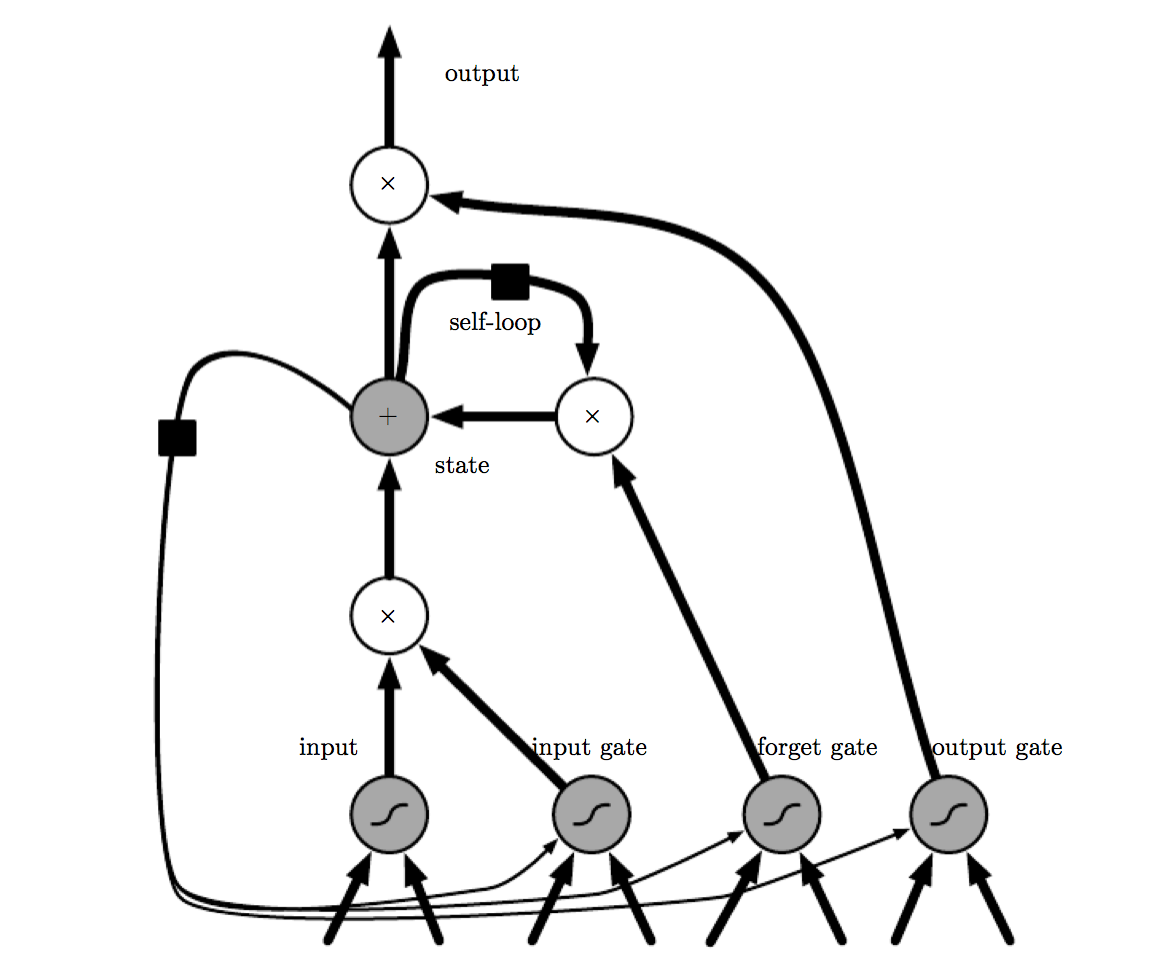
\includegraphics[width=\textwidth]{lstm}
  \caption{Estructura de la compuerta cerrada de una LSTM.
    (Tomado de \cite{goodfellow-et-al-2016})}
  \label{convnet_fig}
\end{figure}



\subsubsection*{Entrenamiento}

TODO
